\section{Interaktive Karte}

In diesem Teil wird die Implementierung der im Abschnitt \ref{sec:analyse-karten} prototypisch erstellten interaktiven Karte mithilfe des JavaScript-APIs von Google Maps entwickelt.

\subsection{Leistung bei der Datenerfassung}

Die interaktive Karte verdankt ihre Langsamkeit vor allem dem Abruf der Sensordaten, der über mehrere Aufrufe an eine sehr langsame API erfolgt.
Tatsächlich dauert es mehr als 2000 Millisekunden, um einfach nur den Standort von 10 Sensoren an einem Standort abzurufen.
Der Grund dafür ist, dass der Backend Service viele Informationen über die Sensoren zurückgibt, was wiederum umfangreiche JOINs in der Datenbank erforderlich macht.

\begin{figure}[H]
  \centering
  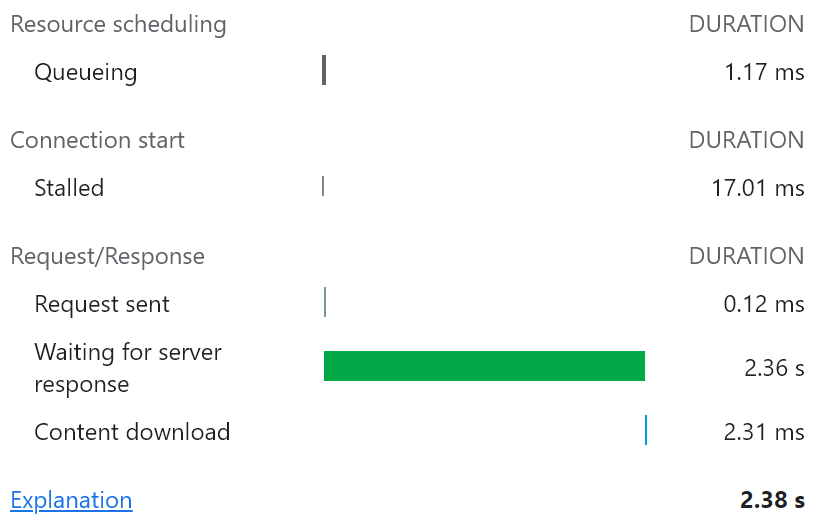
\includegraphics[width=8cm]{api_sensors_global_duration}
  \caption{Durchschnittliche Antwortzeit bei 10 Aufrufen an die Sensor-API}
  \label{fig:api_sensors_global_duration}
\end{figure}

Die Anwendung muss dann für jeden Sensor einen weiteren API-Aufruf tätigen, um dessen Status abzurufen.
Diese Strategie ist für eine interaktive Karte nicht geeignet, da das Hinzufügen von Sensoren die API noch weiter verlangsamen würde.
Es ist eine neue Strategie erforderlich, die es ermöglicht, den Standort und den Status von Tausenden von Sensoren innerhalb einer angemessenen Zeit abzurufen.

Drei Hauptideen wurden ausgewählt.
Da diese Techniken nicht zum direkten Thema der Thesis gehören, werden sie nur kurz beschrieben.

\subsubsection{API-Antwort-Cache}

Der Großteil der derzeit verfügbaren APIs implementiert ein Caching-System für Antworten\cite{redis}.
Wenn ein Benutzer eine Liste aller Sensoren an einem bestimmten \textit{Site} anfordert, wird die Antwort mit einem \ac{TTL} gespeichert und der nächste Benutzer, der die gleiche Liste anfordert, erhält die Antwort aus dem Backup, wenn der \ac{TTL} nicht abgelaufen ist.

\paragraph{Vorteile}
\begin{itemize}
  \item Verringerung der Serverbelastung
  \item Einfache Einrichtung mit ID-basierten Speichersystemen wie z.B. Redis
  \item Kann auf Browserseite im Header der \ac{HTTP}-Antwort einer Anfrage verwaltet werden
\end{itemize}

\paragraph{Nachteile}
\begin{itemize}
  \item Die Antworten sind schneller, aber sie lösen nicht die Tatsache, dass der Benutzer dann für jeden Sensor eine neue Anfrage aufrufen muss
  \item Kann nicht auf der Clientseite implementiert werden, da es zu Inkonsistenzen bei den kritischen Client-Server-Daten kommen kann (Feuer entdeckt)
\end{itemize}

\subsubsection{API mit serverseitiger Statusberechnung} \label{sec:API_serverseitiger_Statusberechnung}

Dieser Ansatz zielt darauf ab, zwei neue API-Endpunkte speziell für die Karte zu erstellen, die den Standort und den Status der \textit{Sites} und die Sensoren eines \textit{Site} abrufen können.

\paragraph{Vorteile}
\begin{itemize}
  \item Relativ einfach einzurichten, ohne Breaking Changes zu verursachen
  \item Der Kunde muss nicht mehr die API aufrufen, um den Status jedes einzelnen Sensors abzufragen, sondern es genügen zwei Anfragen.
\end{itemize}

\paragraph{Nachteile}
\begin{itemize}
  \item fügt hyperspezifische Endpunkte hinzu, wodurch die API komplizierter zu verstehen ist
  \item Die Berechnung des Status eines Sensors ist auf der Serverseite schneller, aber je mehr Sensoren vorhanden sind, desto langsamer ist die Antwort
\end{itemize}

\subsubsection{Kontinuierliche Berechnung mit Big-Data-Ansatz} \label{sec:API_bigdata}

Diese Technik implementiert die vorherige Technik (siehe \ref{sec:API_serverseitiger_Statusberechnung}), außer dass die Berechnung des Status eines bestimmten Sensors in einer temporären Datenbanktabelle gespeichert wird.
Sobald ein Sensor eine Information sendet, wird sein Status parallel zum Hauptprozess neu berechnet und der Eintrag in der Datenbank geändert.
So wird die Abfrage des Status der Sensoren einer \textit{Site} einfach zum Lesen einer Datenbanktabelle.

\paragraph{Vorteile}
\begin{itemize}
  \item Extrem schnelle Antwortzeit, da keine Datenverarbeitung erforderlich ist
  \item Ressourceneffizienz, da die Berechnungen nur für ein bestimmtes Element bei einem bestimmten Ereignis durchgeführt werden
  \item Kann in einer Micro-Service-Architektur isoliert werden
\end{itemize}

\paragraph{Nachteile}
\begin{itemize}
  \item Erfordert einen Fallback, um sicherzustellen, dass die Daten mit der Datenbank konsistent sind
  \item Höhere Entwicklungskosten
\end{itemize}

\subsubsection{Entscheidung}

Zusammen mit dem Backend-Team wurde beschlossen, die letzte Option (siehe \ref{sec:API_bigdata}) in der nächsten Version der Anwendung zu implementieren.
Aus Zeit- und Prioritätsgründen wird jedoch die zweite Option (siehe \ref{sec:API_serverseitiger_Statusberechnung}) implementiert.
Die Nutzung der API ist die gleiche, aber die Leistung ist nicht optimal.

Dadurch konnte die Anzahl der API-Aufrufe, die zuvor linear zur Anzahl der Sensoren an einem Standort war, auf eins reduziert werden.
Die Reaktionszeit ist mit über 1100 Millisekunden für 10 Sensoren immer noch übermäßig hoch, aber diese Lösung ist nur eine Übergangslösung und für die Größe der derzeit in Produktion befindlichen Sites immer noch verwendbar.

\begin{figure}[H]
  \centering
  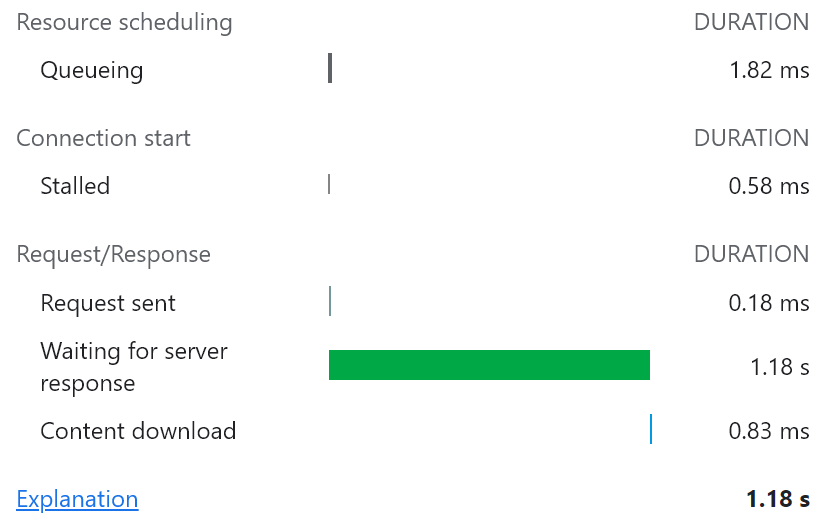
\includegraphics[width=8cm]{api_sensors_map_duration}
  \caption{Durchschnittliche Reaktionszeit für 10 API-Aufrufe, die der Anzeige von Sensoren auf der Karte zugedacht sind}
  \label{fig:api_sensors_map_duration}
\end{figure}

Das Detail der neuen API, das für die Karte gewidmet ist, finden Sie im Anhang \ref{appendix:map-api}.

\subsection{Clustering von \textit{Sites} und Sensoren}

Dieser Abschnitt konzentriert sich auf das Abrufen von Geodaten von \textit{Sites} und Sensoren und deren optimierte Clustering.

\subsubsection{Punkt-Clustering-Algorithmus}

Die Tatsache, dass es zwei mögliche Ebenen von Clustern zwischen \textit{Sites} und Sensoren gibt, erlaubt es nicht, das native Clustering-API von Google Maps zu verwenden, das nur für Punkte mit der gleichen Hierarchie funktioniert.
Wir müssen also die Clustering-Logik selbst entwickeln, indem wir den \ref{fig:map_clustering_flow} flow implementieren.

Es gibt viele Algorithmen für das Clustering von Geopunkten, aber um das Rad nicht neu zu erfinden, wird das mapbox \textit{supercluster}\footnote{Siehe \href{https://github.com/mapbox/supercluster}{https://github.com/mapbox/supercluster}} project verwendet, das im Hintergrund von Google Maps eingesetzt wird.
Diese Open-Source-Javascript-Bibliothek ist sehr populär geworden, da sie Punkte unter dem GeoJSON-Datenstandard\cite{rfc7946} verwaltet und eine unglaubliche Leistung beim Clustern von Millionen von Punkten mit Hilfe eines \textit{gierigen hierarchischen Clustering}-Algorithmus\cite{supercluster} erzielt.

Die Logik hinter diesem Algorithmus besteht darin, die nächstgelegenen Punkte zu bestimmten Punkten anhand eines Radius zu berechnen, um einen neuen Clusterpunkt auf der tiefsten Zoomstufe der interaktiven Karte zu bilden (18 im Fall von Google Maps in der Anwendung von dryad).
Der Algorithmus wiederholt die Operation bei der obersten Zoomstufe mit den Clusterpunkten, bis er bei Zoom 0 angekommen ist.
Auf diese Weise nimmt die Anzahl der zu clusternden Punkte mit abnehmendem Zoom-Level exponentiell ab.
Der Algorithmus erlaubt es auch, sofort die untergeordneten Cluster eines bestimmten Clusters zu erkennen.

\begin{figure}[H]
  \centering
  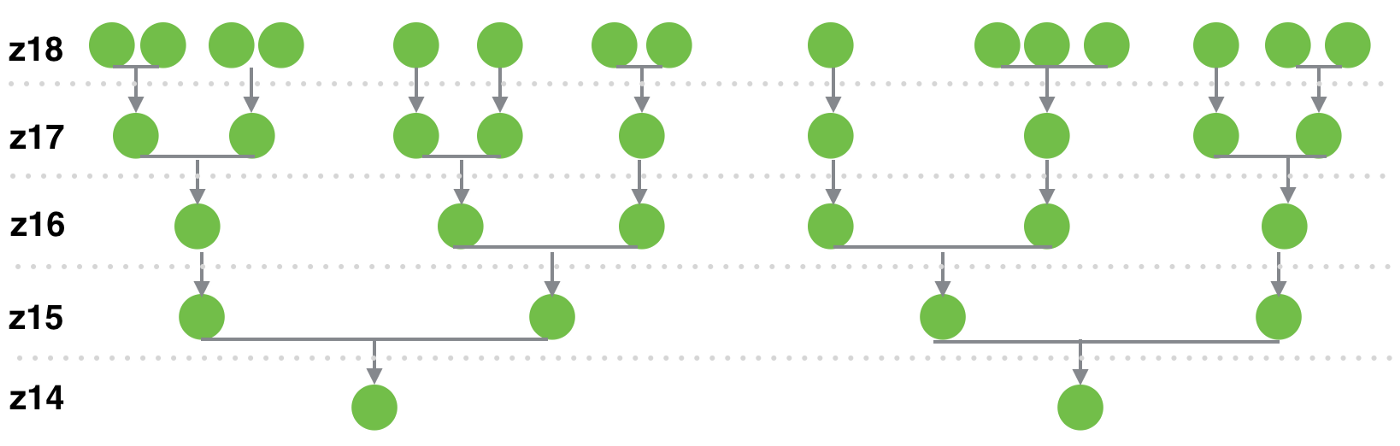
\includegraphics[width=10cm]{supercluster_clustering}
  \caption{Darstellung des Algorithmus \textit{gierigen hierarchischen Clusterings} in Abhängigkeit von der Zoomstufe}
  \label{fig:supercluster_clustering}
\end{figure}

\subsubsection{Abrufen von geospatialen Punkten}

Der Clustering-Algorithmus ist entweder sehr optimiert, aber wenn er beim Laden der Karte durch den Benutzer alle Sensoren clustern soll, muss der Benutzer auf viele zeitraubende \ac{HTTP}-Anfragen warten.
Daher ist es notwendig, die verschiedenen API-Aufrufe nur dann zu tätigen, wenn der Clustering-Algorithmus sie benötigt.
Der Daten-Fetch-Flow kann folgendermaßen schematisiert werden:

\begin{figure}[H]
  \centering
  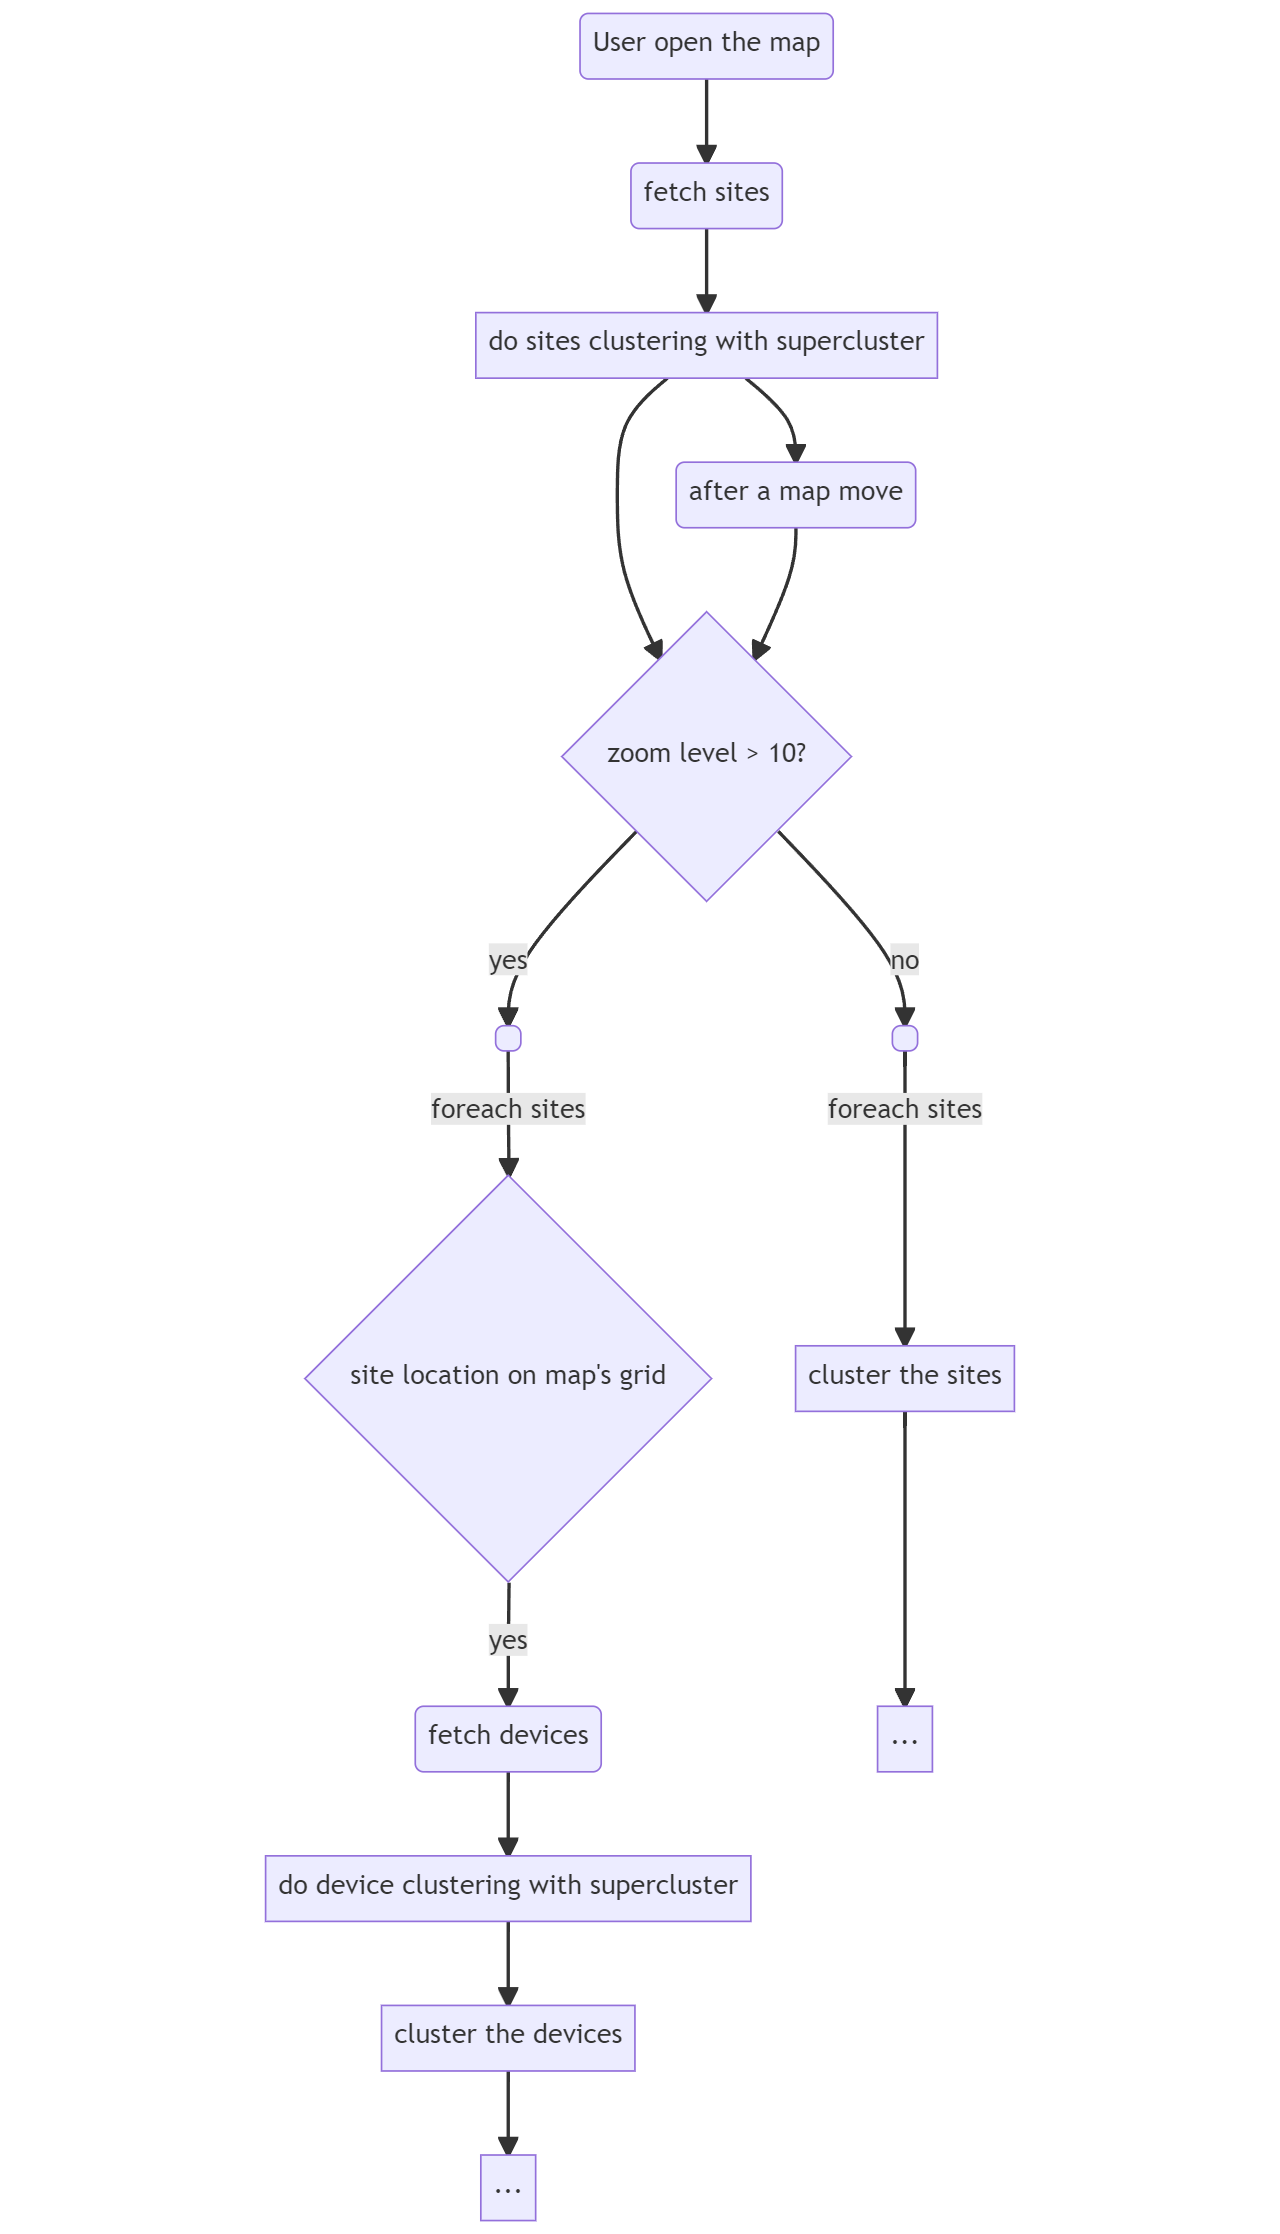
\includegraphics[width=9cm]{map_fetch_flow}
  \caption{Logik der API-Aufrufe bei der Benutzerinteraktion auf der interaktiven Karte}
  \label{fig:map_fetch_flow}
\end{figure}

So erfolgt der Aufruf der API zur Lokalisierung der Sensoren nur, wenn ein Standort isoliert und auf der Karte sichtbar ist und die Zoomstufe größer als 10 ist.

Die Zoomstufe 10 entspricht der Anzeigeebene einer Stadt wie Berlin.
Es wurde intern gesehen, dass es unwahrscheinlich ist, dass ein Kunde jemals eine einzige zu schützende \textit{Site} dieser Größe haben wird.
So wird der API-Aufruf lange vor dem Zeitpunkt erfolgen, an dem die Sensoren einzeln angezeigt werden müssen, sodass die Daten Zeit haben, verarbeitet zu werden.

\subsubsection{Caching von Clustern} \label{sec:clustern_caching}

Die \textit{supercluster}-API ermöglicht es, die Cluster der geladenen Punkte für einen bestimmten Zoom-Level und einen rechteckigen Bereich der Karte namens bbox zu berechnen, der aus den Koordinaten der vier Punkte in diesem Rechteck instanziiert wird.

\begin{lstlisting}[
  language=javascript,
  caption={Vereinfachter Code für das Laden von Punkten und die Berechnung von Clustern mit \textit{supercluster}},
  captionpos=b,
  label={lst:supercluster_example}
]
import Supercluster from "supercluster"

const supercluster = new Supercluster({...options})
supercluster.load(points)

supercluster.getClusters(bbox, zoomLevel) // list of cluster points
\end{lstlisting}

Würde man auf diese Weise die Cluster berechnen, die bei einer Bewegung der Karte auf der Karte angezeigt werden sollen, müsste man die alten Cluster von der Karte entfernen, um die neuen zu zeichnen.
Nur bei vielen Interaktionen, wie z. B. einem kurzen Mausklick, sind die Cluster, die angezeigt werden sollen, bereits auf der Karte vorhanden.
Sie sollten die Aktionen Hinzufügen und Löschen auf der Google Maps-Karte nur dann ausführen, wenn es notwendig ist.
Beachten Sie, dass es notwendig ist, Marker auf der Karte zu entfernen, die nicht sichtbar sind, um die Leistung der interaktiven Karte nicht zu verlangsamen.

Dazu wird eine Wrapperklasse \lstinline{SuperCluster} verwendet.
Diese speichert die auf der Karte angezeigten Cluster im Speicher.
Bei der Berechnung neuer Cluster gibt sie zurück, welche Cluster gelöscht, welche hinzugefügt und welche übrig bleiben.
Diese Cluster werden in der Struktur eines \lstinline{Feature<Point>} aus dem GeoJSON-Standard\cite{rfc7946} angegeben.

\begin{figure}[H]
  \centering
  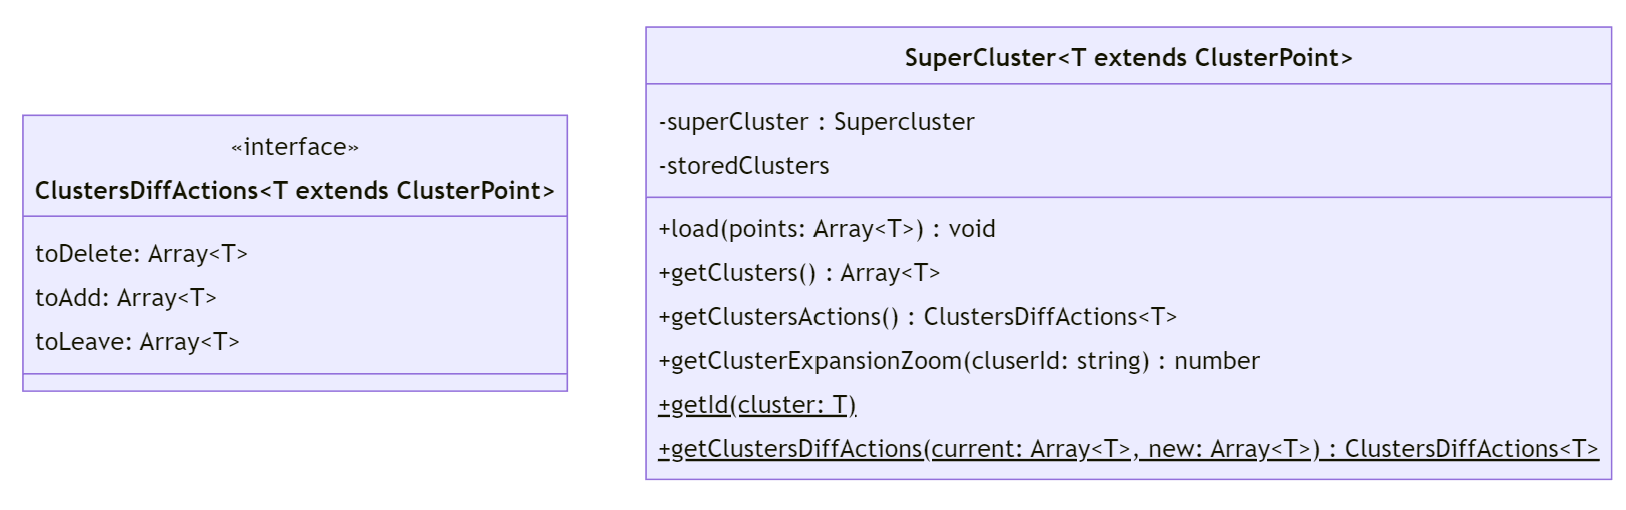
\includegraphics[width=11cm]{class_diagram_supercluster}
  \caption{Class diagramm des \textit{SuperCluster}-Wrappers}
  \label{fig:class_diagram_supercluster}
\end{figure}

Cluster werden im Objekt \lstinline{storedClusters} gespeichert, indem sie durch ihren Längengrad, Breitengrad und Zoomstufe, getrennt durch ein Komma, identifiziert werden.
Zwei Cluster können sich nicht zur selben Zeit am selben Ort befinden, daher ist die Kennung eindeutig.

Die Instanz der Google Maps-Karte wird an den \lstinline{SuperCluster}-Konstruktor übergeben.
So wird der Bereich bbox ist die Zoomstufe bei jedem Aufruf der Methode \lstinline{getClustersActions} automatisch erkannt.

Mit der Methode \lstinline{getClusterExpansionZoom} können Sie die nächste Zoomstufe erfahren, bei der ein Cluster geteilt wird.
Diese Methode ist sehr nützlich für die Implementierung der in \ref{sec:map_interaction} erwähnten Clickinteraktionen.

\subsubsection{Übersetzung und Akkumulierung von Daten in das GeoJSON-Format}

Die Standort- und Sensordaten der API kommen als Array von Elementen des Typs \lstinline{SiteStatus} und \lstinline{SensorNodeStatus} an (siehe \ref{appendix:map-api}).
Wir müssen jede Entität in GeoJSON-Punkte vom Typ \lstinline{Feature<Point>} umwandeln, damit wir sie mit supercluster clustern können.
Der Vorteil der Verwendung eines \lstinline{Feature}-Objekts anstelle eines einfachen \lstinline{Point} liegt darin, dass jede Markierung die notwendigen Informationen enthalten muss, um den Status eines Sensors oder Clusters zu ermitteln, wie im Abschnitt \ref{sec:help_reading_map} beschrieben.
Das Feature-Objekt\footnote{Siehe \href{https://www.rfc-editor.org/rfc/rfc7946\#section-3.2}{https://www.rfc-editor.org/rfc/rfc7946\#section-3.2}} besteht nämlich aus einer geospazialen Information, der zusätzliche \lstinline{properties} hinzugefügt werden können.

Die \lstinline{properties} für \textit{Sites}- und Sensorpunkte sind \lstinline{SiteProperties} bzw. \lstinline{DeviceProperties}, die Sie im Anhang \ref{lst:pointsproperties} finden.
Dann loopen einfach alle Elemente der API-Antwort und wenden eine Mutation auf das Element mittels einer Funktion an, wie im folgenden Beispiel, das ein \lstinline{SiteStatus}-Objekt eingibt und ein \lstinline{Feature<Point, SiteProperties>}-Objekt zurückgibt.

\begin{lstlisting}[
  language=javascript,
  caption={Beispiel für eine Ein-/Ausgabefunktion, die die Übersetzung eines Typs ermöglicht},
  captionpos=b,
  label={lst:toPointConvertion}
]
const getSiteClusterPoint = (site: SiteStatus): Feature<Point, SiteProperties> => {
  const {
    id,
    name,
    fireAlertStatus,
    centerLatitude,
    centerLongitude,
  } = site

  return {
    type: "Feature",
    properties: {
      site_id: id,
      name,
      lat: centerLatitude,
      lng: centerLongitude,
      fire_alert: fireAlertStatus === 0 ? undefined : fireAlertStatus,
      offline: Utils.isOffline(site),
      maintenance: Utils.needsMaintenance(site),
    },
    geometry: {
      type: "Point",
      coordinates: [ centerLongitude, centerLatitude ],
    },
  }
}
\end{lstlisting}

Die Eigenschaften \lstinline{fire_alert}, \lstinline{offline} und \lstinline{maintenance} ermöglichen es, den Status eines \textit{Site} oder Sensors zu erfahren.
Ein Cluster aus mehreren Elementen muss daher auch diese Eigenschaften haben, um seinen Status zu kennen, der die Akkumulation der Eigenschaften der Elemente, aus denen er besteht, widerspiegelt.

Die Eigenschaften \lstinline{map} und \lstinline{reduce} (siehe \href{https://github.com/mapbox/supercluster\#property-mapreduce-options}{https://github.com/mapbox/supercluster\#property-mapreduce-options}) des Objekts \lstinline{options}, die bei der Instanziierung von \lstinline{SuperCluster} übergeben werden können, ermöglichen es, die Eigenschaften jedes Punktes eines berechneten Clusters zu akkumulieren.
Das folgende Beispiel ermöglicht es einem Cluster, die Eigenschaften jedes Sensors zu akkumulieren, um die im Abschnitt \ref{sec:help_reading_map} detailliert beschriebene Priorität zu erfüllen.
Der Cluster hat auch die Eigenschaft \lstinline{devices}, die allen Punkten der Sensoren, aus denen er besteht, entspricht.

\begin{lstlisting}[
  language=javascript,
  caption={\lstinline{SuperCluster}-Akkumulationsoptionen für Sensorcluster},
  captionpos=b,
  label={lst:clustering_reduce_options}
]
const options = {
  map: (props) => ({
    devices: [ props ],
    id: props.id,
    name: props.name,
    fire_alert: props.fire_alert,
    offline: props.offline,
    maintenance: props.maintenance,
  }),
  reduce: (accumulated, props) => {
    const getAccumulatedFireAlert = (): AlertPhases | undefined => {
      if (accumulated.fire_alert) {
        if (accumulated.fire_alert === AlertPhases.PHASE_TWO || props.fire_alert === AlertPhases.PHASE_TWO)
          return AlertPhases.PHASE_TWO
        if (accumulated.fire_alert === AlertPhases.PHASE_ONE)
          return AlertPhases.PHASE_ONE
        return props.fire_alert
      }
      return props.fire_alert
    }

    accumulated.devices = accumulated.devices ? [ ...accumulated.devices, props ] : [ props ]
    accumulated.fire_alert = getAccumulatedFireAlert()
    accumulated.offline = accumulated.offline || props.offline
    accumulated.maintenance = accumulated.maintenance || props.maintenance
  },
}
\end{lstlisting}


\subsection{Rendering von Markern auf Google Maps}

Die verschiedenen Sensoren, Cluster und \textit{Sites} sollen dem Nutzer nun auf einer interaktiven Google-Maps-Karte mithilfe von Markern angezeigt werden.
Dies wird durch die Verwendung der Klasse \lstinline{google.maps.Marker}\footnote{Siehe \href{https://developers.google.com/maps/documentation/javascript/examples/marker-modern}{https://developers.google.com/maps/documentation/javascript/examples/marker-modern}} ermöglicht, die als Parameter ein Icon im \ac{SVG}-Format übernehmen kann.
Mithilfe der Klasse \lstinline{google.maps.Size} kann diesem Marker eine relative Größe zugewiesen werden.
Auf diese Weise ist es sehr einfach, Marker auf der Karte anzuzeigen, wie im \ref{fig:map_markers_size} beschrieben.

\subsubsection{Ansatz mit funktionaler Programmierung} \label{sec:implementation_functional}

In einem ersten Schritt wurde ein \ac{POC} mithilfe funktionaler Programmierung entwickelt.
Diese war erfolgreich, da die verschiedenen Sensoren, Cluster und \textit{Sites} auf der Karte angezeigt und beim Verschieben oder Zoomen aktualisiert wurden.

Obwohl der Ansatz ziemlich naiv war, da für jeden neu berechneten Cluster die gesamte Instanziierung eines Markers erneut durchgeführt werden musste (selbst wenn derselbe Marker bereits zuvor instanziiert worden war, was beim Vergrößern und Verkleinern der Karte häufig vorkommt), war keine Leistungsverlangsamung auf PC- oder mobilen Browsern zu erkennen.
Die Strategie schien aufzugehen, aber schon bald überschnitten sich der Code und die vielen Funktionsaufrufe, sodass das Hinzufügen jedes neuen Features chaotisch wurde.

Wie Sie weiter unten sehen können, wird der Funktionscode für eine solch komplexe Logikverwaltung in einen Programmteil verwandelt, der das Verständnis des Kontrollflusses sehr schwierig macht.
Diese Nicht-Architektur wird umgangssprachlich als Spaghetti-Programmierung bezeichnet, da sie sich in alle Richtungen ausdehnt\cite{spaghetti}.

\begin{figure}[H]
  \centering
  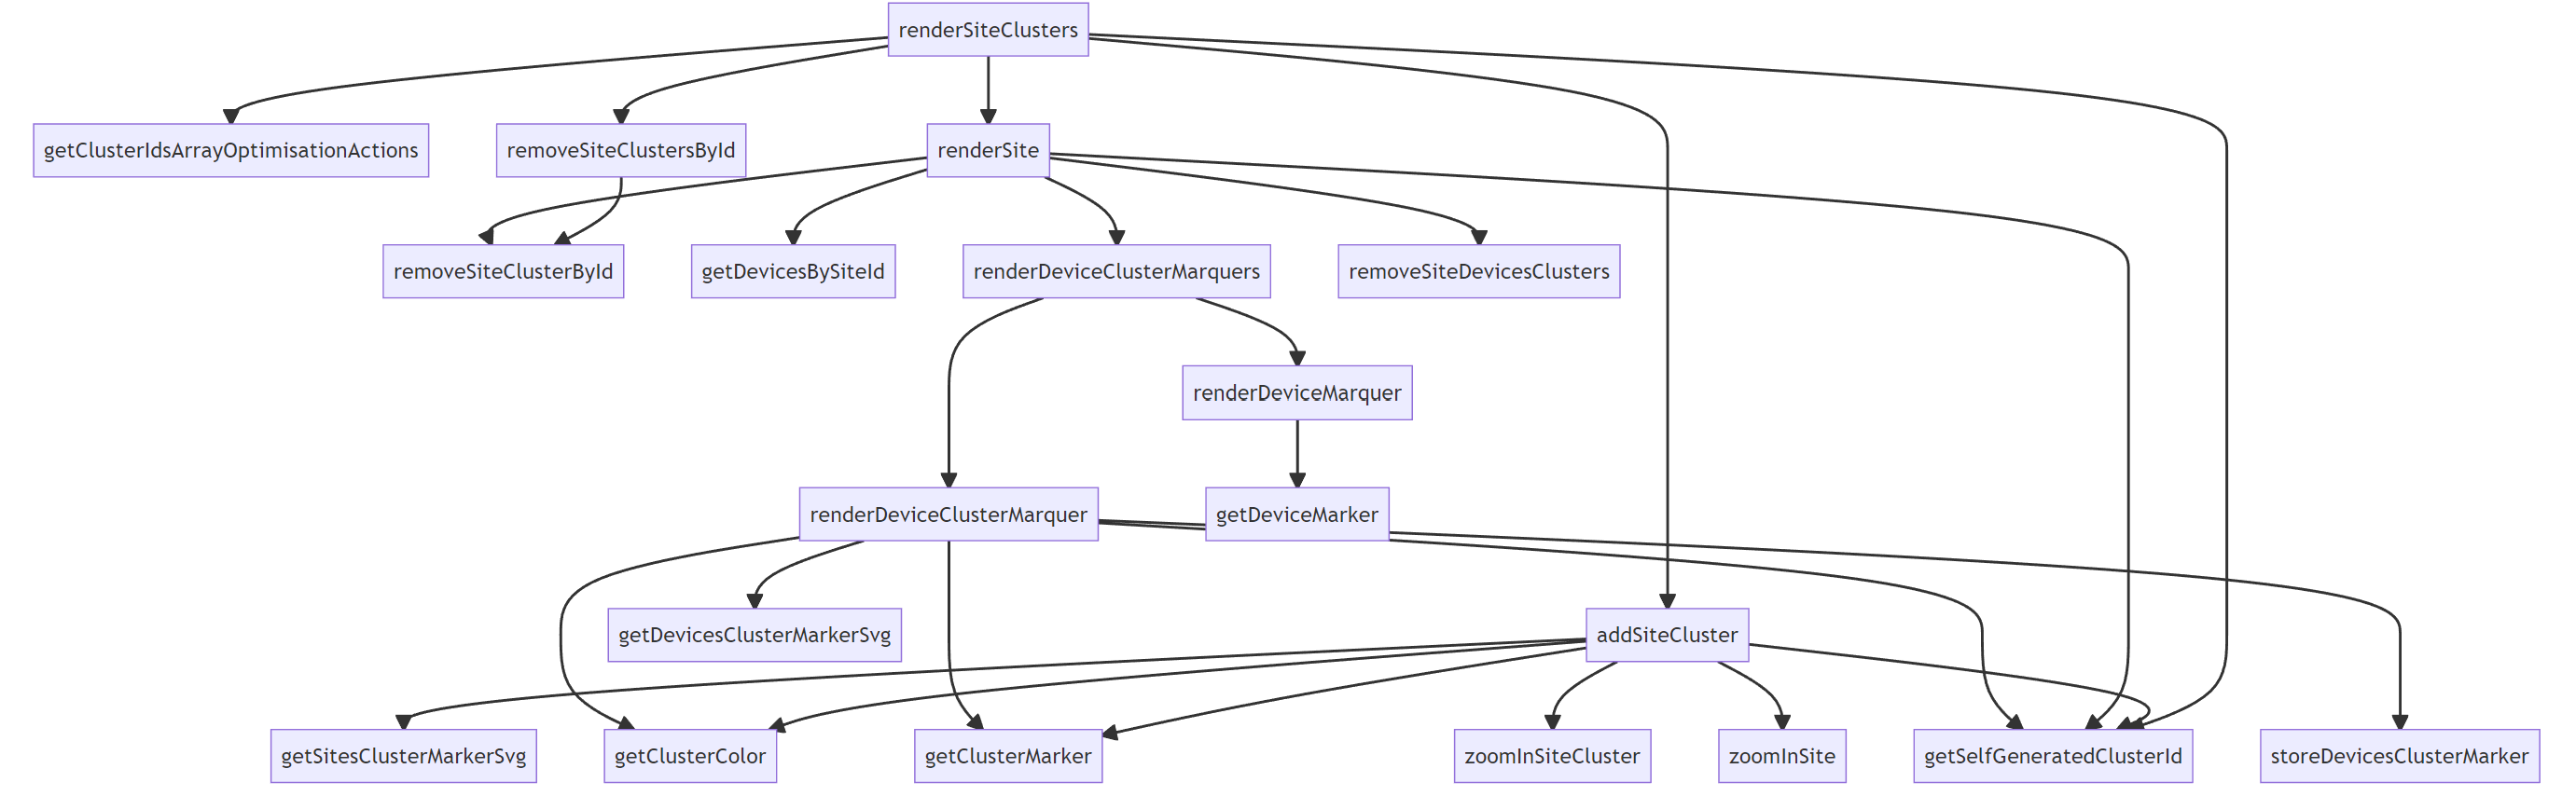
\includegraphics[width=23cm,angle=90]{map_functions_poc}
  \caption{Schematische Darstellung der Funktionsaufrufe für die Anzeige von Markern, die für den \ac{POC} verwendet wurde}
  \label{fig:map_functions_poc}
\end{figure}

Der POC-Code zeigt auch die Entstehung von Funktionen, die sich mit der Verwaltung bestimmter Entitäten befassen und andere gemeinsame Funktionen in Form von Vererbung nutzen.
Diese Art von Architektur lässt direkt an eine Lösung denken, die mit \ac{OOP} entwickelt wurde.

\subsubsection{Ansatz mit der \ac{OOP}}

Der \ac{OOP}-Ansatz des \ac{POC} ermöglicht es, den Code in einzelne Klassen zu isolieren, die sich mit einem sehr konkreten Aspekt der Kartendarstellung befassen (\lstinline{SensorNodeMarker}, \lstinline{SiteArea}, \lstinline{SitesCluster}), während der globale Code aus übergeordneten Klassen (\lstinline{Marker}, \lstinline{Cluster}, \lstinline{DeviceMarker}) wiederverwendet wird.
Das folgende Klassendiagramm zeigt die Architektur des \ac{POC}, in dem die Verwaltung von Markern, die Reichweite einer \textit{Site} und die Verwaltung von Benutzerinteraktionen implementiert sind.

\begin{figure}[H]
  \centering
  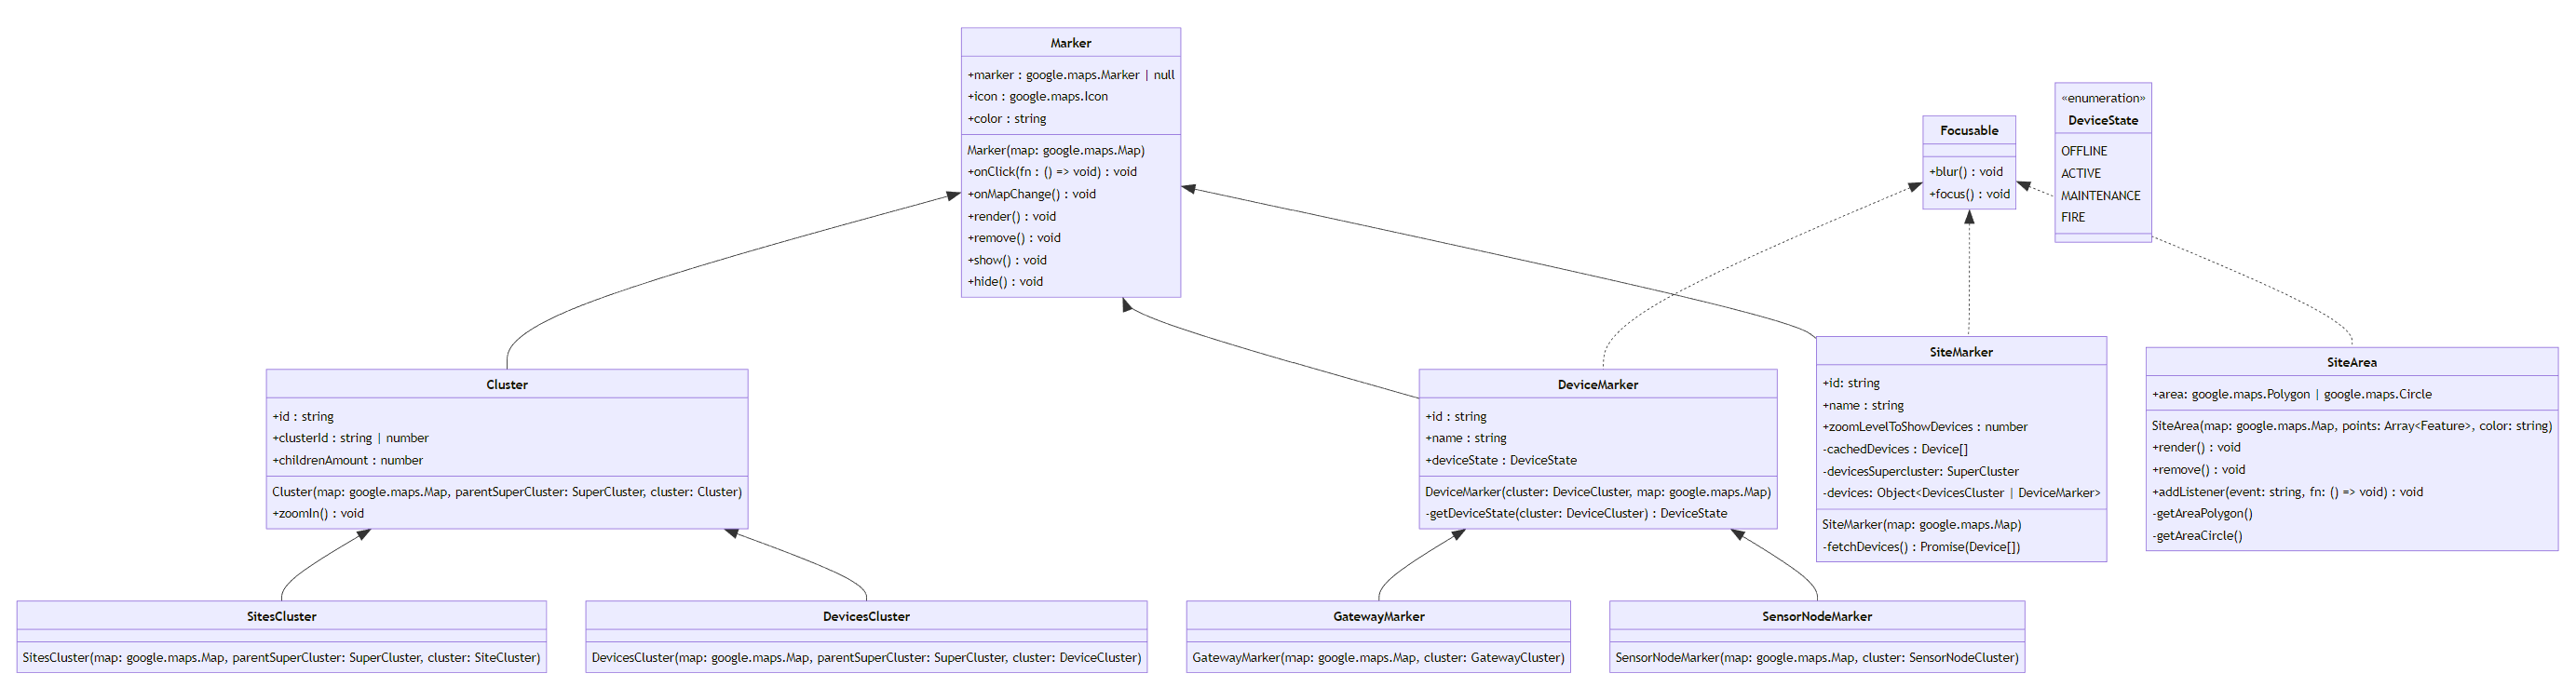
\includegraphics[width=24cm,angle=90]{markers_class_diagramm}
  \caption{Class diagrams des funktionalen POC}
  \label{fig:markers_class_diagramm}
\end{figure}

\subsubsection{Leistung des Marker-Renderings auf der Karte}

Wie im Abschnitt \ref{sec:implementation_functional} beschrieben, muss die Instanziierung eines Markers auf der Karte für jeden neu anzuzeigenden Sensor ausgeführt werden, auch wenn dieser bereits zuvor angezeigt wurde.
Das ist auf unseren Tools kein Leistungsproblem, aber es könnte auf einem viel weniger leistungsfähigen Mobiltelefon sein, wie es bei einigen Kunden in der Welt üblich ist.
Um diese unnötige Berechnung zu vermeiden, werden die instanziierten Marker jeder \textit{Site} und jedes \textit{Site}-Clusters (\lstinline{SiteMarker}, \lstinline{SitesCluster}) in einem Javascript-Objekt mit einem Schlüssel gespeichert, der auf die gleiche Weise wie im Abschnitt \ref{sec:clustern_caching} generiert wird.
Die gleiche Logik wird für die Marker der einzelnen Sensoren und Sensorcluster (\lstinline{DeviceMarker}, \lstinline{DevicesCluster}) verwendet.

Auf diese Weise wird jeder Marker für jede unterschiedliche Zoomstufe nur einmal instanziiert.
Mit den Methoden \lstinline{render} und \lstinline{remove} der Klasse \lstinline{Marker} können Sie den Marker einfach zur Google Maps-Instanz hinzufügen oder ihn wieder entfernen mithilfe der \lstinline{setMap} Methode\footnote{Siehe \href{https://developers.google.com/maps/documentation/javascript/markers}{https://developers.google.com/maps/documentation/javascript/markers}}.

\begin{lstlisting}[
  language=javascript,
  caption={Vereinfachter Code für das Hinzufügen und Entfernen eines Markers auf einer Google Maps Karte},
  captionpos=b,
  label={lst:marker_render_remove}
]
class Marker {
  // ...
  public render(): void {
    this.marker.setMap(this.map)
  }

  public remove(): void {
    this.marker.setMap(null)
  }
  // ...
}
\end{lstlisting}

Auf diese Weise werden die Ressourcen, die beim mehrmaligen Hinein- und Herauszoomen verbraucht werden, deutlich reduziert, da keine Berechnungen mehr erforderlich sind, wenn ein bereits vorhandener Marker angezeigt wird.
